\documentclass[pdf]{beamer}
\usepackage[utf8]{vietnam}
\usepackage{amsmath}
\usepackage{amssymb}
\usepackage[utf8]{inputenc}
\usepackage{algorithm,algorithmic}
\usepackage{subfig}
\usepackage{color}
\usepackage{colortbl}
\mode<presentation>{\usetheme{Madrid}}
%\usecolortheme{whale}

%% preamble
\title{Biterm Topic Model}
%\subtitle{Mô hình Biterm}
\author{Nguyễn Bá Cương}
\institute[]
{
	School of Information and Communication Technology
	Hanoi University of Science and Technology\\
}
\date[VLC 2017] % (optional)
{Data Science Lab , 2017}
\begin{document}
	
	%% title frame
	\begin{frame}
	\titlepage
\end{frame}

%\begin{frame}{Nội dung}
%\tableofcontents
%\end{frame}
%
%\AtBeginSection[]
%{
%\begin{frame}{Nội dung}
%\tableofcontents[currentsection]
%\end{frame}
%}


%%%%%%%%%%%%%%%%%%%%%%%%%%%%%%%%%%%%%%%%%%%

\begin{frame}{Tập dữ liệu NYT, K =50, đô đo perplexity}
%	K = 100, sử dụng độ đo perplexity 
\begin{columns}[T] % align columns
	\begin{column}{.50\textwidth}
		\begin{figure}
			\subfloat[Online Gibbs sampling]{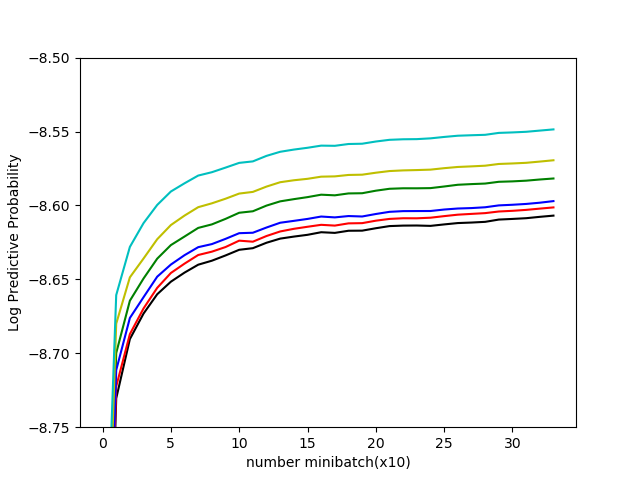
\includegraphics[width=1.1\textwidth]{nyt50gibb.png}}
		\end{figure}
	\end{column} %
	\hfill%	
	\begin{column}{.50\textwidth}
		\begin{figure}
			\subfloat[Online VB]{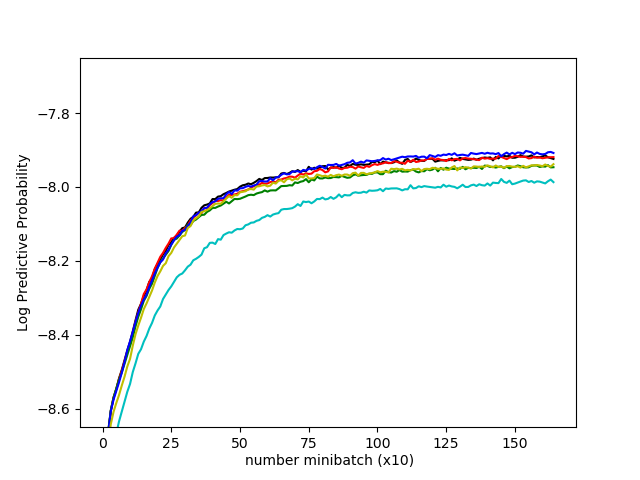
\includegraphics[width=1.1\textwidth]{nyt50vb.png}}
		\end{figure}				
	\end{column} %
\end{columns}
\begin{center}
	
\includegraphics[width=1\textwidth]{menu.png}	
\end{center}
\end{frame}

\begin{frame}{Tập dữ liệu NYT, K = 50, sử dụng độ đo NPMI }
\begin{columns}[T] % align columns
\begin{column}{.50\textwidth}
	\begin{figure}
		\subfloat[Online Gibbs sampling]{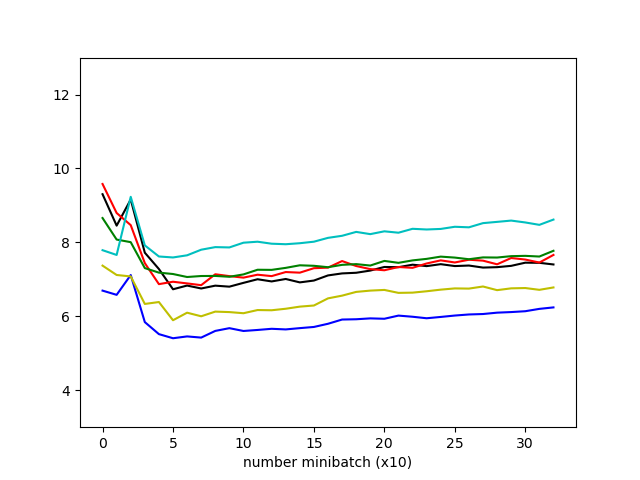
\includegraphics[width=1.1\textwidth]{npmi_nyt_50_gibbs.png}}
	\end{figure}
\end{column} %
\hfill%	
\begin{column}{.50\textwidth}
	\begin{figure}
		\subfloat[Online VB]{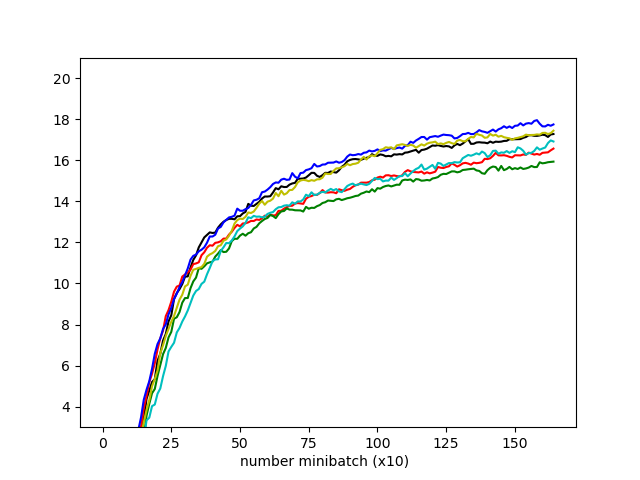
\includegraphics[width=1.1\textwidth]{npmi_nyt_50_vb.png}}
	\end{figure}				
\end{column} %
\end{columns}
\begin{center}

\includegraphics[width=1\textwidth]{menu.png}	
\end{center}
\end{frame}

\begin{frame}{Tập dữ liệu NYT, K = 100, sử dụng độ đo perplexity }

\begin{columns}[T] % align columns
	\begin{column}{.50\textwidth}
		\begin{figure}
			\subfloat[Online Gibbs sampling]{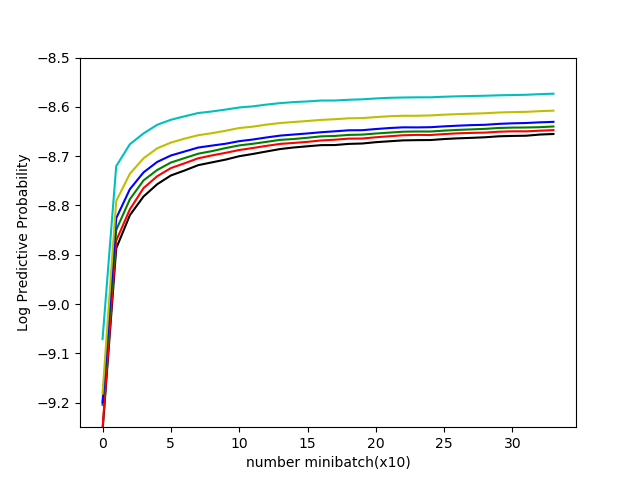
\includegraphics[width=1.1\textwidth]{nyt100gibb.png}}
		\end{figure}
	\end{column} %
	\hfill%	
	\begin{column}{.50\textwidth}
		\begin{figure}
			\subfloat[Online VB]{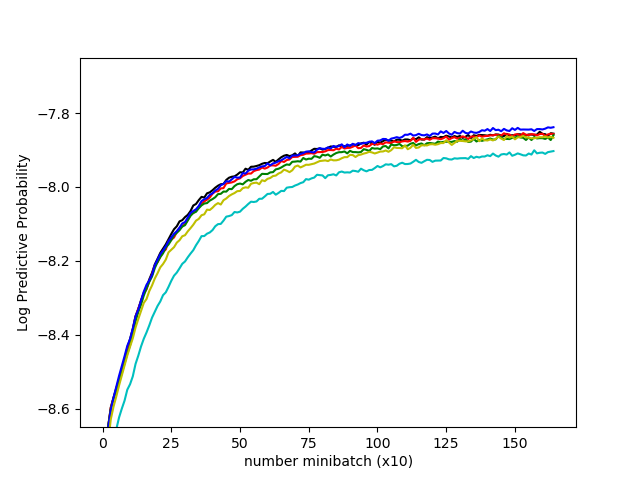
\includegraphics[width=1.1\textwidth]{nyt100vb.png}}
		\end{figure}				
	\end{column} %
\end{columns}
\begin{center}
	
\includegraphics[width=1\textwidth]{menu.png}	
\end{center}
\end{frame}


\begin{frame}{Tập dữ liệu NYT, K = 100, sử dụng độ đo NPMI }
\begin{columns}[T] % align columns
\begin{column}{.50\textwidth}
	\begin{figure}
		\subfloat[Online Gibbs sampling]{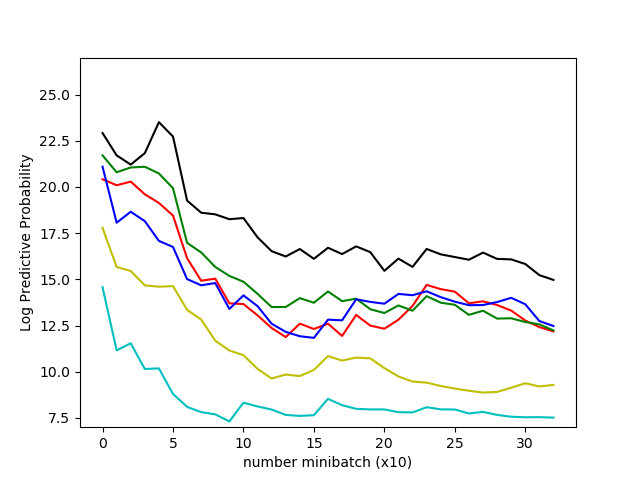
\includegraphics[width=1.1\textwidth]{npmi_nyt_100_gibbs.png}}
	\end{figure}
\end{column} %
\hfill%	
\begin{column}{.50\textwidth}
	\begin{figure}
		\subfloat[Online VB]{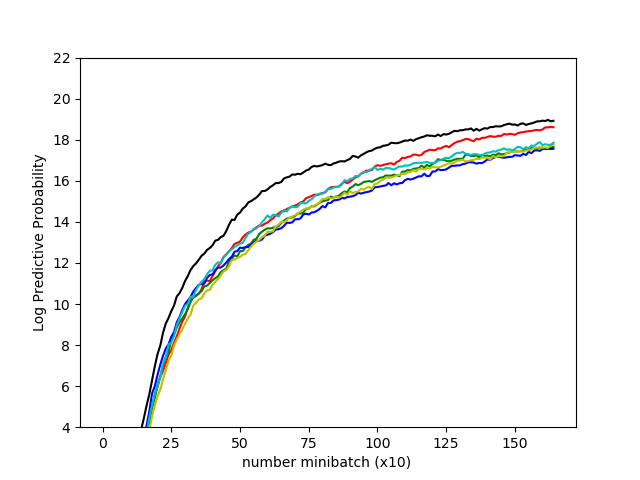
\includegraphics[width=1.1\textwidth]{npmi_nyt_100_vb.png}}
	\end{figure}				
\end{column} %
\end{columns}
\begin{center}

\includegraphics[width=1\textwidth]{menu.png}	
\end{center}
\end{frame}

\begin{frame}{Tập dữ liệu NYT, K =150, đô đo perplexity}
%	K = 100, sử dụng độ đo perplexity 
\begin{columns}[T] % align columns
\begin{column}{.50\textwidth}
\begin{figure}
	\subfloat[Online Gibbs sampling]{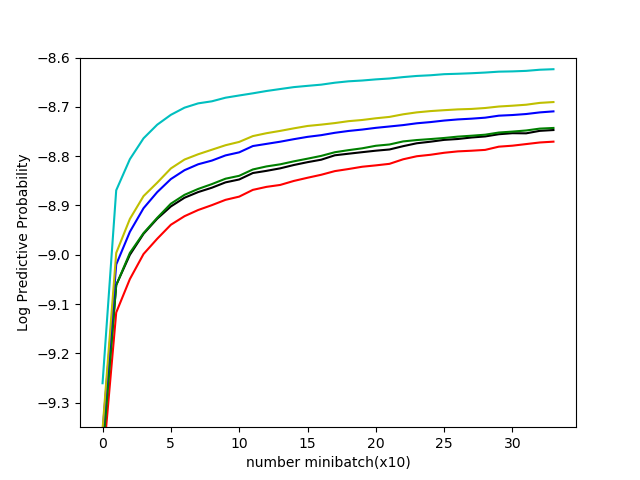
\includegraphics[width=1.1\textwidth]{nyt150gibb.png}}
\end{figure}
\end{column} %
\hfill%	
\begin{column}{.50\textwidth}
\begin{figure}
	\subfloat[Online VB]{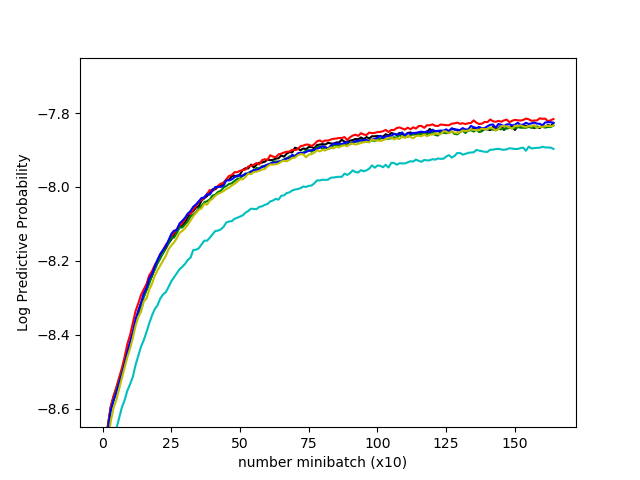
\includegraphics[width=1.1\textwidth]{nyt150vb.png}}
\end{figure}				
\end{column} %
\end{columns}
\begin{center}

\includegraphics[width=1\textwidth]{menu.png}	
\end{center}
\end{frame}

\begin{frame}{Tập dữ liệu NYT, K = 150, sử dụng độ đo NPMI }
\begin{columns}[T] % align columns
\begin{column}{.50\textwidth}
\begin{figure}
\subfloat[Online Gibbs sampling]{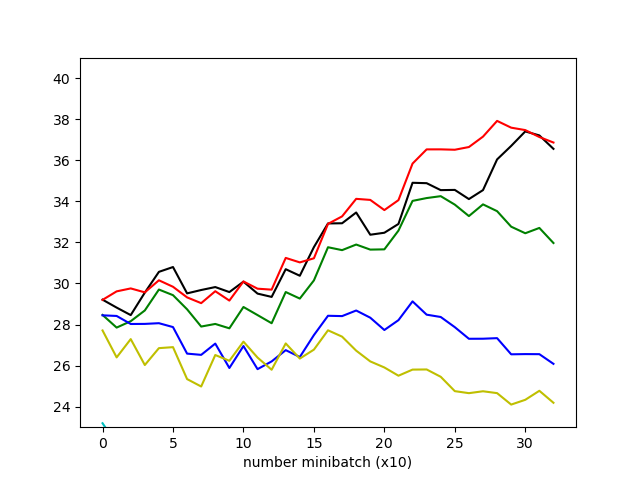
\includegraphics[width=1.1\textwidth]{npmi_nyt_150_gibbs.png}}
\end{figure}
\end{column} %
\hfill%	
\begin{column}{.50\textwidth}
\begin{figure}
\subfloat[Online VB]{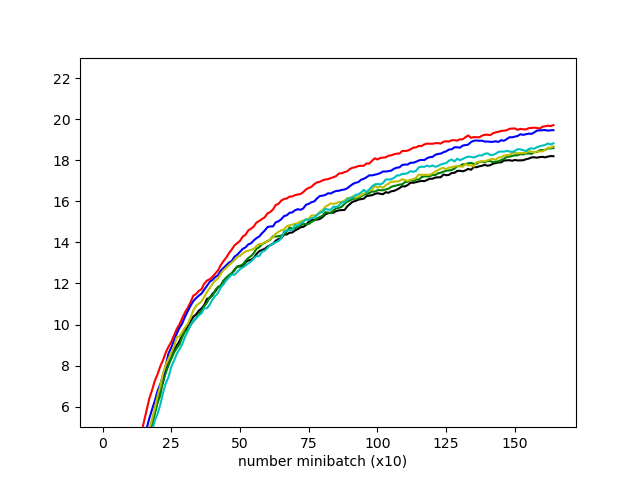
\includegraphics[width=1.1\textwidth]{npmi_nyt_150_vb.png}}
\end{figure}				
\end{column} %
\end{columns}
\begin{center}

\includegraphics[width=1\textwidth]{menu.png}	
\end{center}
\end{frame}


\begin{frame}{Tập dữ liệu NYT, K =200, đô đo perplexity}
%	K = 100, sử dụng độ đo perplexity 
\begin{columns}[T] % align columns
\begin{column}{.50\textwidth}
\begin{figure}
\subfloat[Online Gibbs sampling]{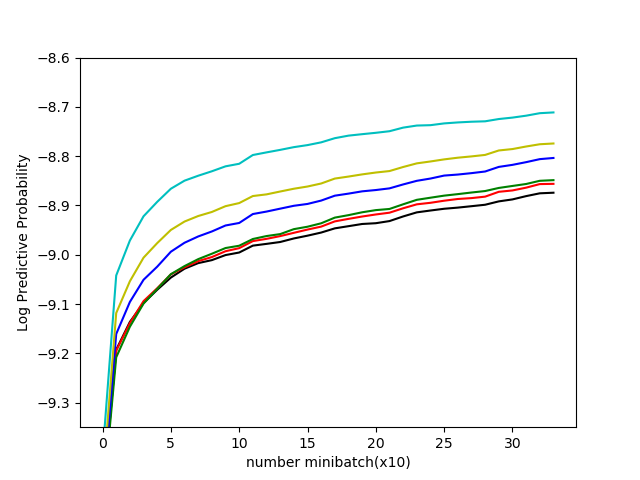
\includegraphics[width=1.1\textwidth]{nyt200gibb.png}}
\end{figure}
\end{column} %
\hfill%	
\begin{column}{.50\textwidth}
\begin{figure}
\subfloat[Online VB]{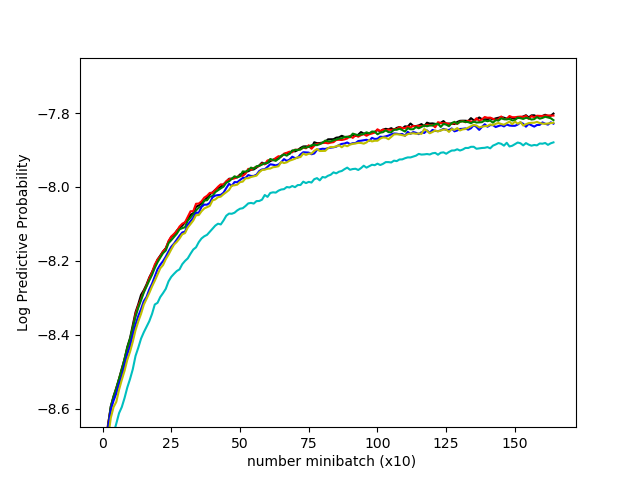
\includegraphics[width=1.1\textwidth]{nyt200vb.png}}
\end{figure}				
\end{column} %
\end{columns}
\begin{center}

\includegraphics[width=1\textwidth]{menu.png}	
\end{center}
\end{frame}

\begin{frame}{Tập dữ liệu NYT, K = 200, sử dụng độ đo NPMI }
\begin{columns}[T] % align columns
\begin{column}{.50\textwidth}
\begin{figure}
\subfloat[Online Gibbs sampling]{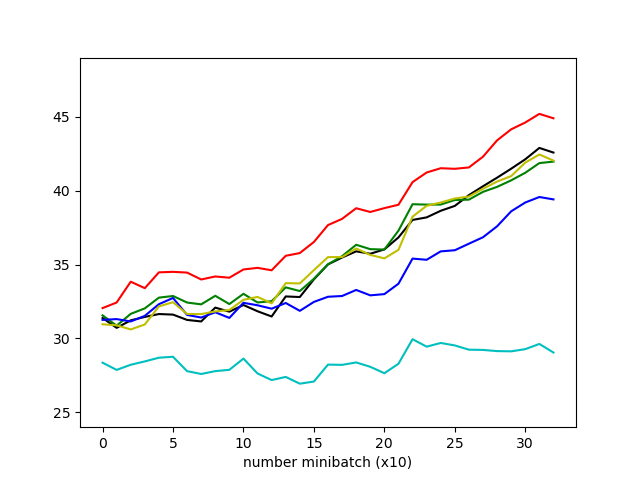
\includegraphics[width=1.1\textwidth]{npmi_nyt_200_gibbs.png}}
\end{figure}
\end{column} %
\hfill%	
\begin{column}{.50\textwidth}
\begin{figure}
\subfloat[Online VB]{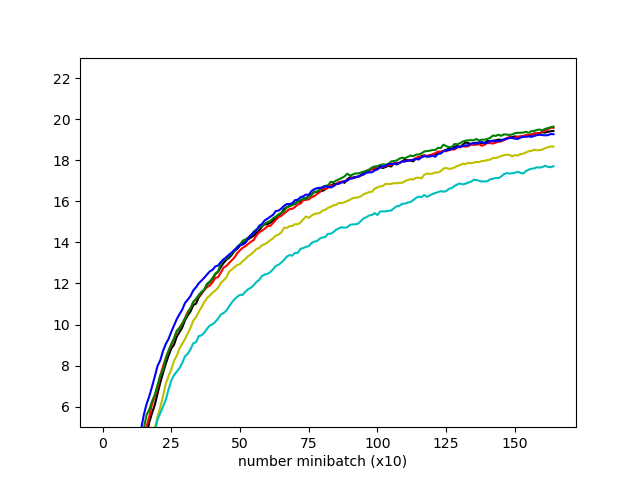
\includegraphics[width=1.1\textwidth]{npmi_nyt_200_vb.png}}
\end{figure}				
\end{column} %
\end{columns}
\begin{center}

\includegraphics[width=1\textwidth]{menu.png}	
\end{center}
\end{frame}

\end{document}
